\section{Device Software}




\subsection{Overview}

The device software makes up the bulk of the work done within this project. The basic algorithm devised by Y Hu et al is mostly unmodified, with the modifications limited primarily to the communication of data between devices. This work can broadly be split into three sections; the data input handler, the inter-FPGA communication, and the library data read-out. The data input handler interfaces with the host software and distributes the input data across the system. The inter-FPGA communication controls the algorithm's execution to guarantee synchronisation across the multiple devices. The result data handler returns the overlap libraries produced by each pixel via the UART interface with the host. In order to explain the design of these three sub-systems it is important to understand the over-arching aims of the device software. The top level of this system can be seen in figure  \ref{fig:tld}. Each device contains a data Input/Output (IO) handler as well as small modifications to the global controller. Through maintaining the same structure as far as possible, the implementation minimises the impact of cross-device interfacing on each device's operations.

What this approach does in terms of the algorithm is split work in a uniform fashion, increasing the work done by a single pixel, but keeping the total work done per FPGA the same. This can be explained by viewing an all-against-all comparison as a matrix of comparisons.




$
\text{Comparison Matrix} =  
\begin{pmatrix}
  F(a_{1},a_{1}) & F(a_{1},a_{2})  & \cdots & F(a_{1},a_{n}) \\
  F(a_{2},a_{1}) & F(a_{2},a_{2})  & \cdots & F(a_{2},a_{n}) \\
  \vdots  & \vdots   & \ddots & \vdots   \\
  F(a_{n},a_{1}) & F(a_{n},a_{2}) & \cdots & F(a_{n},a_{n}) \\
 \end{pmatrix}  
 $
 
 
Within this matrix each pixel does one column of work, performing the comparison between 1 common sequence and all other sequences. However, there are no true dependencies within this matrix, any comparison can be carried out in any order. In the original comparison engine, the movement of data around the chip was the driving factor, so each pixel started with it's own sequence, and then used data forwarded around the ring network. This can be understood within the matrix as each pixel starting on it's entry in the leading diagonal of the matrix and then working up the matrix, looping at the top down to the bottom. In this way all the comparisons happen together in lockstep.

Splitting this algorithm across mutliple devices is complex due to this fact however, as currently pixels only do the same number of comparisons as there are on the board. In the newer design one of these pixels will still do the comparisons with all the sequences from the entire cluster, and as such the link between number of pixels present and  number of comparison cycles must be broken. Each device can then be viewed as a rectangular matrix, which when concatenated form the previous complete matrix as shown below for 3 devices.




\begin{align*}
\text{FPGA}_0
 &=
 \begin{pmatrix}
  F(a_{1},a_{1}) & F(a_{1},a_{2})  & \cdots & F(a_{1},a_{\frac{n}{3} }) \\
  F(a_{2},a_{1}) & F(a_{2},a_{2})  & \cdots & F(a_{2},a_{\frac{n}{3} }) \\
  \vdots  & \vdots & \ddots & \vdots   \\
  F(a_{n},a_{1}) & F(a_{n},a_{2})  & \cdots & F(a_{n},a_{\frac{n}{3} }) \\
 \end{pmatrix} \\
\text{FPGA}_1
 &=
 \begin{pmatrix}
  F(a_{1},a_{\frac{n}{3}+1}) & F(a_{1},a_{\frac{n}{3}+2})  & \cdots & F(a_{1},a_{\frac{2n}{3}}) \\
  F(a_{2},a_{\frac{n}{3}+1}) & F(a_{2},a_{\frac{n}{3}+2})  & \cdots & F(a_{2},a_{\frac{2n}{3}}) \\
  \vdots  & \vdots & \ddots & \vdots   \\
  F(a_{2n},a_{\frac{n}{3}+1}) & F(a_{n},a_{\frac{n}{3}+2})  & \cdots & F(a_{n},a_{\frac{2n}{3}})
 \end{pmatrix} \\
 \text{FPGA}_2
 &=
 \begin{pmatrix}
  F(a_{1},a_{\frac{2n}{3}+1}) & F(a_{1},a_{\frac{2n}{3}+2})  & \cdots & F(a_{1},a_{n}) \\
  F(a_{2},a_{\frac{2n}{3}+1}) & F(a_{2},a_{\frac{2n}{3}+2})  & \cdots & F(a_{2},a_{n}) \\
  \vdots  & \vdots & \ddots & \vdots   \\
  F(a_{2n},a_{\frac{2n}{3}+1}) & F(a_{n},a_{\frac{2n}{3}+2})  & \cdots & F(a_{n},a_{n})
 \end{pmatrix} \\
 \\
\text{Comparison Matrix} &= \text{FPGA}_0 \parallel \text{FPGA}_1 \parallel \text{FPGA}_2 \\
\end{align*} 


This shows there are now $\frac{n}{y}$ pixels per device with y devices, but each pixel still does n comparisons. This idea will be revisited later in discussions of other future work.
 
The decision was made to favour a shared clock, lockstep operation design for this implementation, the reason for this is that the ring network design has a natural dependancy loop. This would mean any discrepancy in throughput would cause the system to  hang both for the slowest element of the system but also for communication within the system and would require significant local data storage to mitigate local sources of latency such as long memory accesses on a single FPGA. The lock step design introduces a problem of both guaranteeing coherence across the system as well as practical limitations on clock speed. These practical limitations will be discussed in the implementation section.



The algorithm provided gives a number of important features that must be kept, stream processing and independent logical elements being the most important. 
\begin{sidewaysfigure}[p]
  \centering
  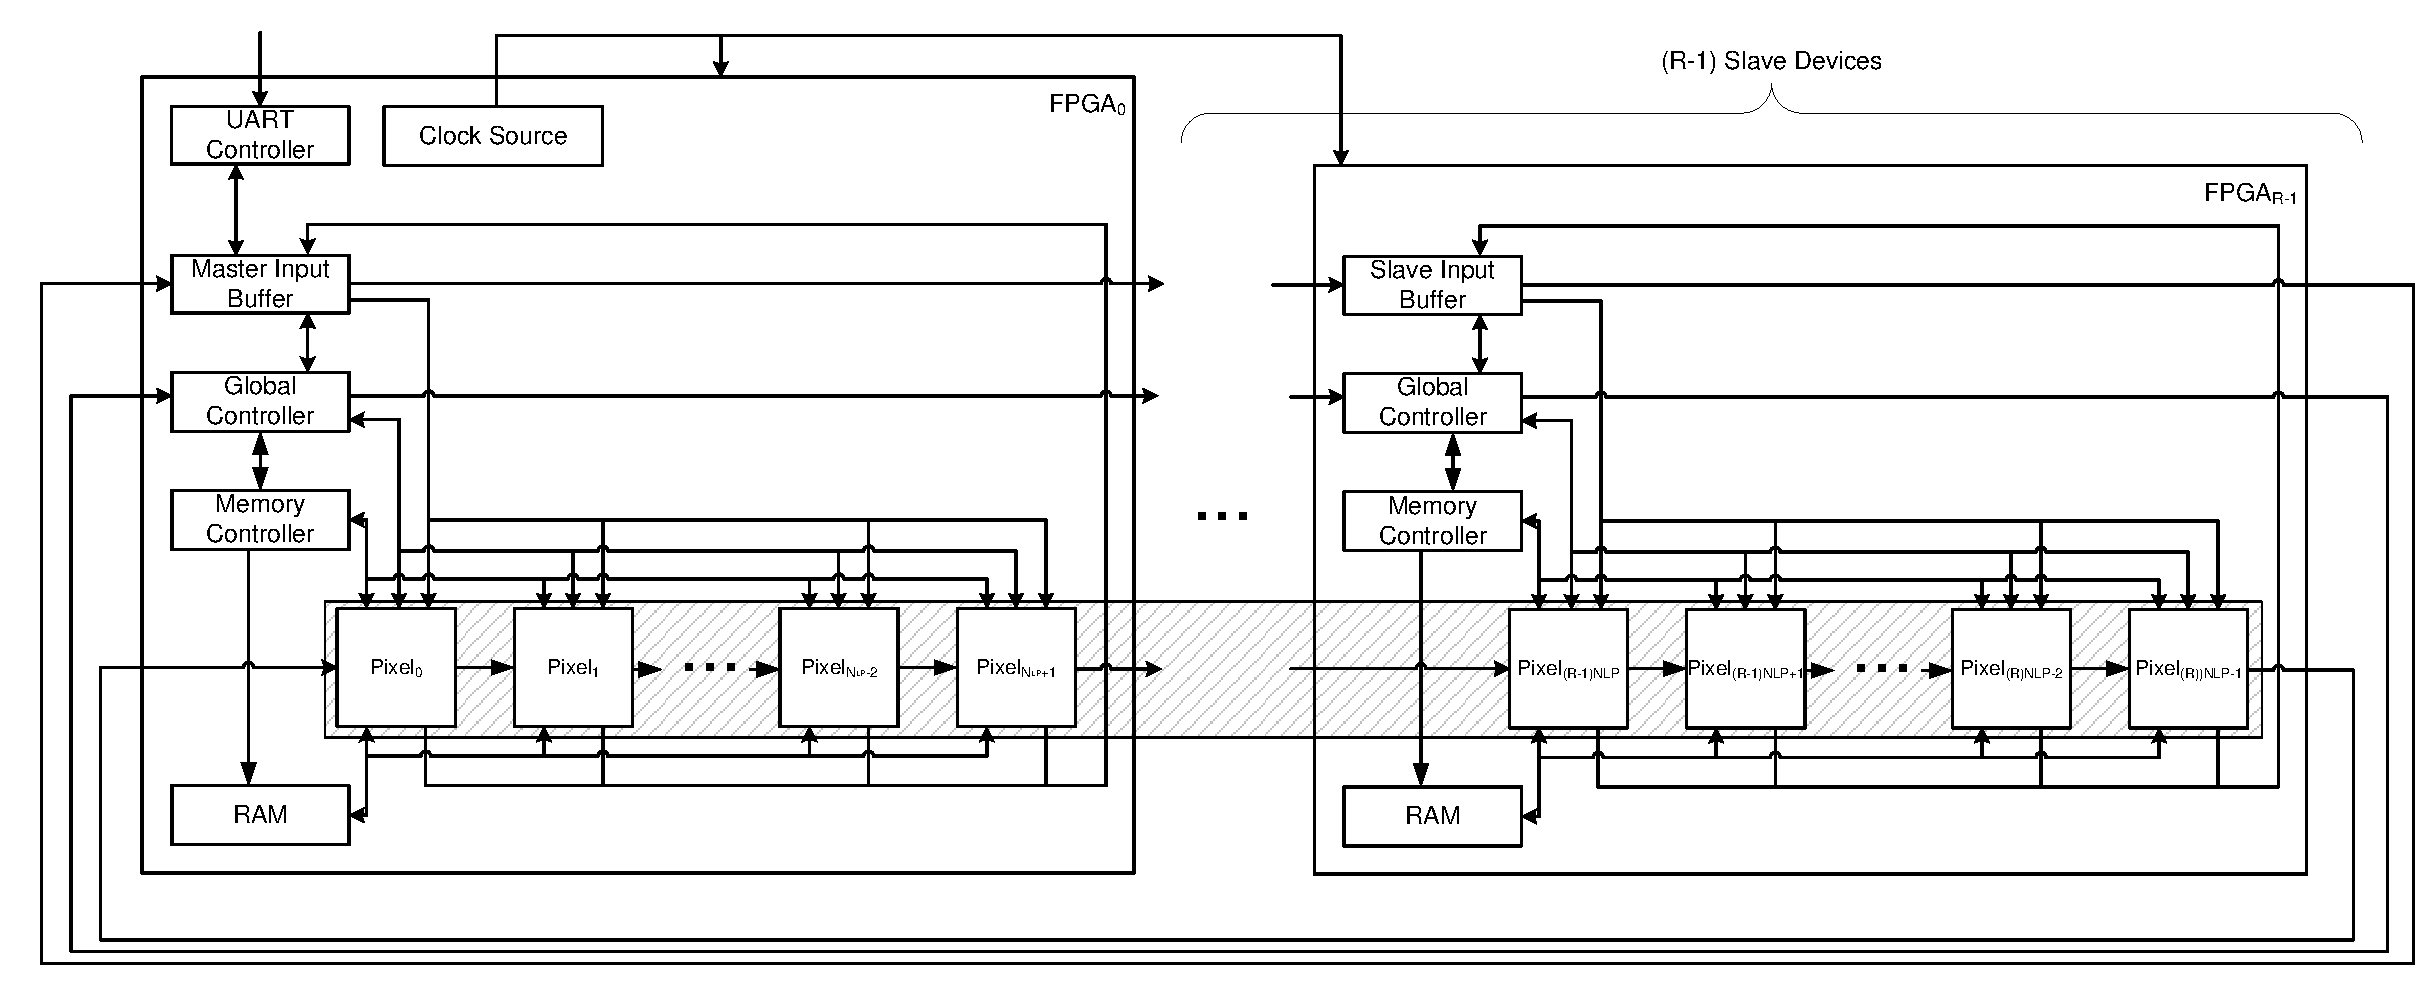
\includegraphics[width=\textheight]{./figs/MFPGA.pdf}
  \caption{Top Level Diagram, 1 Host, R-1 Slave Devices}
  \label{fig:tld}
\end{sidewaysfigure}


\subsection{Data Input Handler}
All the data transfers with the host machine are done via one connection, this is present only on a master FPGA, the other devices received data forwarded around the ring network. It is important however, that the processing happens in lock step, as a result the input data must be available on all FPGAs at the same time. This can be done either through communication between FPGAs or through strict control of the data path. As communication is relatively expensive (due to the high latency of sending signals around the ring network) a fixed latency approach has been chosen. As an over-arching design decision, all signals sent between devices are clocked out and in with no logic. This guarantees the maximum allowance for the data path between devices. 

\subsubsection{The Master UART Connection}
Present only on the master device, the UART interface works at the $\pm$13~volt RS232 specification with the data transfer protocol shown in figure \ref{fig:UART}. The UART controls both the incoming data to be processed and the outgoing data reported to the host. The format of the incoming data is a stream ordered first by read order then by pixel order. The data rate achieved by this interface is up to 1~Mbaud, this is 1 million symbols per second. In the context of  a device that can fit up to 100 pixels as discussed in the complexity analysis of the algorithm, this is significantly faster than necessary. The primary goals of the UART connection is fast enough data rates with low error rates. This is achieved with the oversampled interface. This means for a 1~MBaud system running on  a device with a faster clock, each data bit is sampled multiple times, thus reducing error rates. 
\begin{figure}[!h]
  \centering
  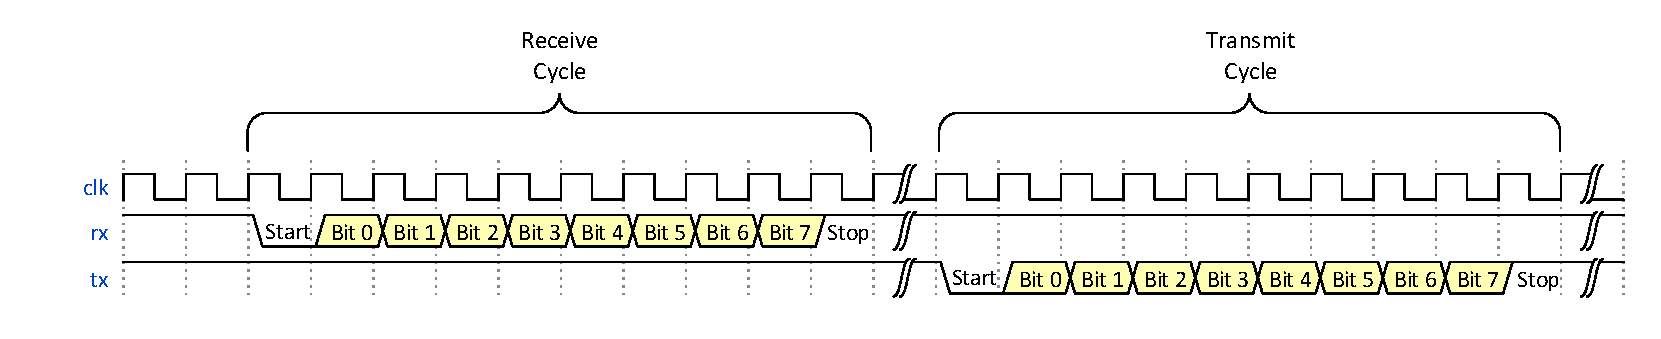
\includegraphics[width=\textwidth]{./figs/UART.pdf}
  \caption{UART Interface Protocol}
  \label{fig:UART}
\end{figure}


The UART controller on the device is designed as a separate module with a simple interface. The reason for this is that if necessary, different external interfaces can replace the UART if necessary. This would be common when implementing the design different hardware which may only have connections for protocols like USB or PCI-Express. In the case of this project an external piece of code was used to interface with the UART standard, this was done as UART interfaces are a standard piece of code and there is little value in reproducing this work.


\subsubsection{Distribution of Input Data}
\begin{figure}[!h]
  \centering
  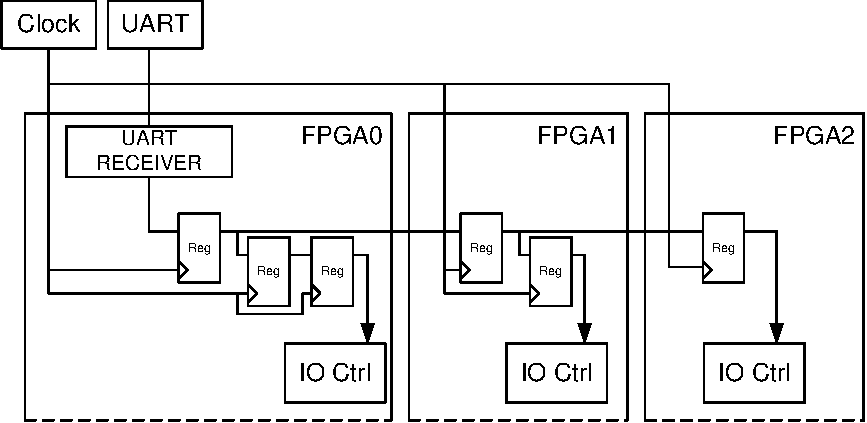
\includegraphics[width=0.8\textwidth]{./figs/input_delay.pdf}
  \caption{Input Delay System Example for 3 Devices}
  \label{fig:delay}
\end{figure}
One of the keys to the lock-step design is ensuring that all the input data appears available to the processor across all devices at the same time. This can be ensured by a simple system of delay registers. This system is shown in figure \ref{fig:delay}, it ensures that all FPGA input adaptors receives the data in lock step. Technically this requires the forwarding of more data than necessary, as data for all pixels reach all FPGAs, as well as invalid data being forwarded with an invalid flag. However, removing this redundancy could not shorten the delay and complicates the logic so it was decided to be preferable to complex logic. The output of this delay cycle is identical across all devices, an 8 bit data chunk with a valid signal going in to the data format translator. The result of this process is a latency of N cycles, where N is the number of devices in the cluster. It is important to note that latency is not an issue in terms of the end speed of the cluster, as it will be hidden during the processing time and is relatively negligible. 






\subsubsection{Data Format Translation}
As discussed earlier, the UART used to input data (and the interface to forward the data between FPGAs) consists of a byte based transmission system. This means data comes in 4 pixels at a time, however the system requires 2 bits to be sent to each pixel in parallel. This requires a complex data width adaptation. This is achieved by clocking data into a wide register 8 bits at a time, and then writing it out to a First In First Out (FIFO) memory structure at the correct bit width. The memory structure adds a small amount of processing flexibility in the case that data is coming in faster than can be processed. In this project the FIFO can store all input data, this is possible due to the fact the comparison engine is very logic element intensive but not memory intensive. A correctly designed FIFO maps to a memory bits on chip, a separate resource to the logic utilisation. As discussed earlier, for a 9 pixel design over 80\% of the logic elements are used on a DE0 device, but less than 1\% of the memory is used. The translation system is a relatively complex translation as is shown in figure \ref{fig:translator}. It is important to note that this width adaptor requires more than 1 pixel per device, otherwise the input adaptor register will be overwritten by a single input twice in a single cycle.

\begin{figure}[!h]
  \centering
  \includegraphics[width=0.9\textwidth]{./figs/input_adaptor.pdf}
  \caption{Input Adaptor, N$_{LP}$-Number of Local Pixels, N$_{TP}$-Number of Total Pixels}
  \label{fig:translator}
\end{figure}



\subsection{Inter-FPGA Communication}

Inter-FPGA communication provides both algorithm synchronisation and extension of the ring network. As shown in figure \ref{fig:tld} the global controller on each device communicates and the ring network communicates.

The extension of the ring network is the most simple, the communication that would normally happen forwarding suffix data between pixels is routed across the GPIO ports as described in the hardware section. Algorithmically this is identical to the original implementation but limits the clock speed due to data transfer rates. This interface is an important limiting factor for the design. The number of connectors between the devices for the ring network is 4 bits for every parallel string being forwarded, this quickly reaches the limits of the number of connectors available. 


The global controller interface is more complex due to the non-fixed nature of the state machine. The state machine for the original algorithm is shown in figure \ref{fig:ctrlfsm}. It can be seen, the only conditional transitions are on input data being available, and checking for pixels to complete. The other transitions are all determined by fixed length states. 


\begin{figure}[!h]
  \centering
  \includegraphics[width=\textwidth]{./figs/ctrl_fsm.pdf}
  \caption{Algorithm Global Controller Finite State Machine}
  \label{fig:ctrlfsm}
\end{figure}


The transition for moving into the read state is conditional on the data being available, as is covered in the previous section, measures have been taken to ensure this happens identically on all devices. The transition from the Wait for All state to Idle state is more difficult however. All pixels must report ready to the controller before the state can proceed. This is very difficult to do across several FPGAs fast, so instead a distributed mechanism has been designed. Each device has all it's pixels report, when all pixels on the master report  it forwards a done signal. Each slave then forwards this signal only when its own pixels are done. When the master receives the done signal back, it then sends a proceed signal and waits a fixed length of time, each slave forwards this signal immediately and waits for 1 fewer cycles. In this way it is guaranteed they count down together. Finally at the end of the countdown they proceed to the next step.

The net result of this in terms of cycles per comparison is that one cycle through the state machine (which corresponds to 1 new piece of data) is increased by $2 \times $the number of pixels. This protocol lowers the speed of comparisons in cycle count, but allows for the fast shared clock. The impact of this will be studied in the testing and evaluation sections. 





\subsection{Result Data Handler}

The result data in the algorithm is stored on a per pixel basis in a library of complex data structures. This library is shown in the listing below. These library entries are known as overlap seeds.


 \begin{center}

 \begin{minipage}{\textwidth}
\lstset{language=python, numbers=left, showspaces=false,
    showstringspaces=false, tabsize=4, breaklines=true, captionpos=b, numbersep=5pt }
\begin{lstlisting}[frame=single,caption=Result Data Format, label=listing:record]
	TYPE SEED IS RECORD
		posi   : RD_INT_TYPE; -- range 0 to READ_LENGTH
		rota   : PIXEL_INT_TYPE; --range 0 to PIXEL_COUNT
		score  : EDDI_INT_TYPE; -- range 0 to REDUNDANCY + 1
		chk_wt : WAIT_INT_TYPE; -- range 0 to INFIX_LENGTH
		bases  : BASE_VECT; -- array 0 to 2 REDUNDANCY + 1
		lock   : STD_LOGIC; 
	END RECORD;
\end{lstlisting}
 \end{minipage}
\end{center}
This data structure is highly dependant on the parameters of the comparison engine and therefore the size is variable. Each library has a parameterisable number of entries and there is one library per pixel. To write this data out across the UART 3 processes must take place. First the data must be gathered per deice and formatted for transfer, then the data must be gathered on the master device, finally the data must be sent out across the UART.
\begin{figure}[!h]
  \centering
  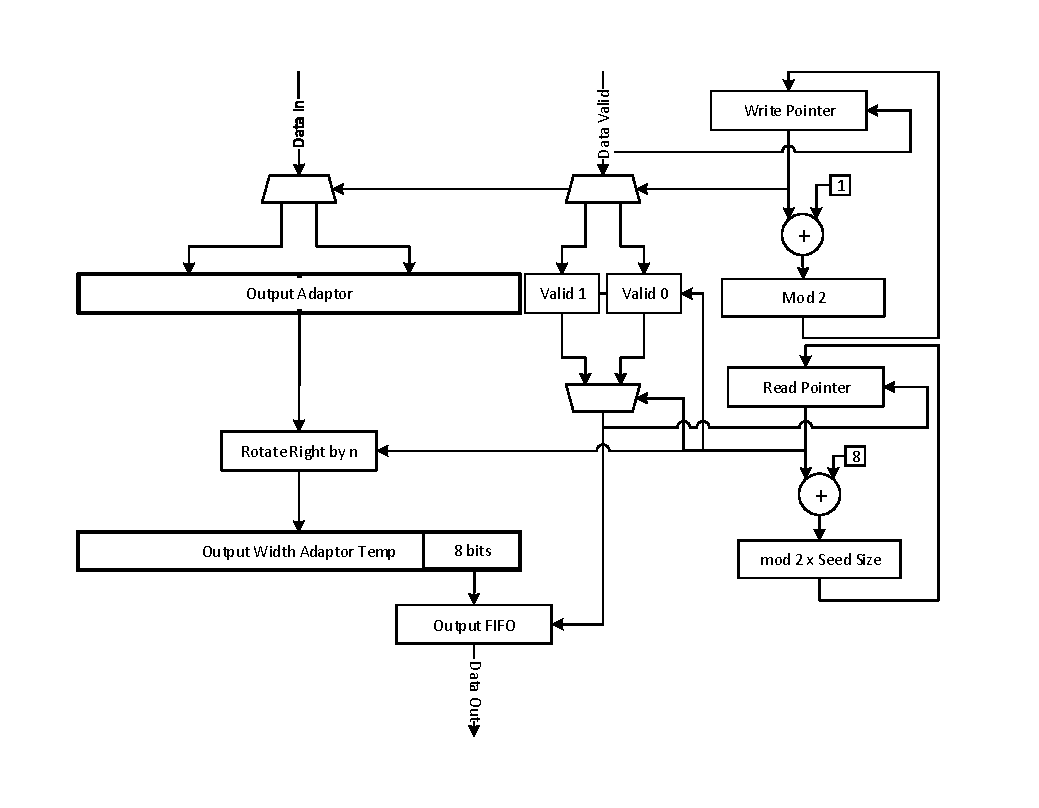
\includegraphics[width=\textwidth]{./figs/output_adaptor.pdf}
  \caption{Output Width Adaptor}
  \label{fig:owa}
\end{figure}

The first stage requires the record to be flattened into a single vector data type. The IO controller on each device then cycles through each pixel requesting their records until they report the end. This then creates a local copy of the libraries together, however this is formed of very large data types that are not suitable for transferring off-chip. Another data width adaptation is required to allow communication between devices, shown in figure \ref{fig:owa}. 


Having translated the current library data into a transferrable format this has to transferred across the ring network. Inter-FPGA communication is already quite high, requiring a large amount of connections so it is best to re-use the data forwarding connections that were used for the input data. The time multiplexing of this connection can safely be used with no effect on performance. The data on the ring network must be transferred in a fixed order to allow reconstruction of the library on the host, this is done by transferring all data from the first slave, followed by an end signal. Each slave in the network forwards the data and uses the stop signal as a prompt to append their own data. The master FPGA caches this data and transmits it over UART, appending it's own library. The impact of caching the full library on one device is small. As covered earlier, memory usage is already extremely low and the library data by nature is only a small fraction of the input data.



